%                                                                 aa.dem
% AA vers. 9.0, LaTeX class for Astronomy & Astrophysics
% demonstration file
%                                                       (c) EDP Sciences
%-----------------------------------------------------------------------
%
%\documentclass[referee]{aa} % for a referee version
%\documentclass[onecolumn]{aa} % for a paper on 1 column
%\documentclass[longauth]{aa} % for the long lists of affiliations
%\documentclass[rnote]{aa} % for the research notes
%\documentclass[letter]{aa} % for the letters
%\documentclass[bibyear]{aa} % if the references are not structured
%                              according to the author-year natbib style

% \documentclass[]{aa}
\documentclass[traditabstract, longauth]{aa}

\usepackage{graphicx}
\usepackage{txfonts}
\usepackage{url}
\usepackage{xcolor}
\usepackage{listings}
\usepackage{import}
\usepackage{fancyvrb}
\usepackage{color}
\usepackage[utf8]{inputenc}
\usepackage{inconsolata}

% comment these out if you already import them in main.tex
\makeatletter
\def\PY@reset{\let\PY@it=\relax \let\PY@bf=\relax\let\PY@ul=\relax \let\PY@tc=\relax\let\PY@bc=\relax \let\PY@ff=\relax}
\def\PY@tok#1{\csname PY@tok@#1\endcsname}
\def\PY@toks#1+{\ifx\relax#1\empty\else\PY@tok{#1}\expandafter\PY@toks\fi}
\def\PY@do#1{\PY@bc{\PY@tc{\PY@ul{\PY@it{\PY@bf{\PY@ff{#1}}}}}}}
\def\PY#1#2{\PY@reset\PY@toks#1+\relax+\PY@do{#2}}

\expandafter\def\csname PY@tok@w\endcsname{\def\PY@tc##1{\textcolor[rgb]{0.73,0.73,0.73}{##1}}}
\expandafter\def\csname PY@tok@c\endcsname{\let\PY@it=\textit\def\PY@tc##1{\textcolor[rgb]{0.25,0.50,0.50}{##1}}}
\expandafter\def\csname PY@tok@cp\endcsname{\def\PY@tc##1{\textcolor[rgb]{0.74,0.48,0.00}{##1}}}
\expandafter\def\csname PY@tok@k\endcsname{\let\PY@bf=\textbf\def\PY@tc##1{\textcolor[rgb]{0.00,0.50,0.00}{##1}}}
\expandafter\def\csname PY@tok@kp\endcsname{\def\PY@tc##1{\textcolor[rgb]{0.00,0.50,0.00}{##1}}}
\expandafter\def\csname PY@tok@kt\endcsname{\def\PY@tc##1{\textcolor[rgb]{0.69,0.00,0.25}{##1}}}
\expandafter\def\csname PY@tok@o\endcsname{\def\PY@tc##1{\textcolor[rgb]{0.40,0.40,0.40}{##1}}}
\expandafter\def\csname PY@tok@ow\endcsname{\let\PY@bf=\textbf\def\PY@tc##1{\textcolor[rgb]{0.67,0.13,1.00}{##1}}}
\expandafter\def\csname PY@tok@nb\endcsname{\def\PY@tc##1{\textcolor[rgb]{0.00,0.50,0.00}{##1}}}
\expandafter\def\csname PY@tok@nf\endcsname{\def\PY@tc##1{\textcolor[rgb]{0.00,0.00,1.00}{##1}}}
\expandafter\def\csname PY@tok@nc\endcsname{\let\PY@bf=\textbf\def\PY@tc##1{\textcolor[rgb]{0.00,0.00,1.00}{##1}}}
\expandafter\def\csname PY@tok@nn\endcsname{\let\PY@bf=\textbf\def\PY@tc##1{\textcolor[rgb]{0.00,0.00,1.00}{##1}}}
\expandafter\def\csname PY@tok@ne\endcsname{\let\PY@bf=\textbf\def\PY@tc##1{\textcolor[rgb]{0.82,0.25,0.23}{##1}}}
\expandafter\def\csname PY@tok@nv\endcsname{\def\PY@tc##1{\textcolor[rgb]{0.10,0.09,0.49}{##1}}}
\expandafter\def\csname PY@tok@no\endcsname{\def\PY@tc##1{\textcolor[rgb]{0.53,0.00,0.00}{##1}}}
\expandafter\def\csname PY@tok@nl\endcsname{\def\PY@tc##1{\textcolor[rgb]{0.63,0.63,0.00}{##1}}}
\expandafter\def\csname PY@tok@ni\endcsname{\let\PY@bf=\textbf\def\PY@tc##1{\textcolor[rgb]{0.60,0.60,0.60}{##1}}}
\expandafter\def\csname PY@tok@na\endcsname{\def\PY@tc##1{\textcolor[rgb]{0.49,0.56,0.16}{##1}}}
\expandafter\def\csname PY@tok@nt\endcsname{\let\PY@bf=\textbf\def\PY@tc##1{\textcolor[rgb]{0.00,0.50,0.00}{##1}}}
\expandafter\def\csname PY@tok@nd\endcsname{\def\PY@tc##1{\textcolor[rgb]{0.67,0.13,1.00}{##1}}}
\expandafter\def\csname PY@tok@s\endcsname{\def\PY@tc##1{\textcolor[rgb]{0.73,0.13,0.13}{##1}}}
\expandafter\def\csname PY@tok@sd\endcsname{\let\PY@it=\textit\def\PY@tc##1{\textcolor[rgb]{0.73,0.13,0.13}{##1}}}
\expandafter\def\csname PY@tok@si\endcsname{\let\PY@bf=\textbf\def\PY@tc##1{\textcolor[rgb]{0.73,0.40,0.53}{##1}}}
\expandafter\def\csname PY@tok@se\endcsname{\let\PY@bf=\textbf\def\PY@tc##1{\textcolor[rgb]{0.73,0.40,0.13}{##1}}}
\expandafter\def\csname PY@tok@sr\endcsname{\def\PY@tc##1{\textcolor[rgb]{0.73,0.40,0.53}{##1}}}
\expandafter\def\csname PY@tok@ss\endcsname{\def\PY@tc##1{\textcolor[rgb]{0.10,0.09,0.49}{##1}}}
\expandafter\def\csname PY@tok@sx\endcsname{\def\PY@tc##1{\textcolor[rgb]{0.00,0.50,0.00}{##1}}}
\expandafter\def\csname PY@tok@m\endcsname{\def\PY@tc##1{\textcolor[rgb]{0.40,0.40,0.40}{##1}}}
\expandafter\def\csname PY@tok@gh\endcsname{\let\PY@bf=\textbf\def\PY@tc##1{\textcolor[rgb]{0.00,0.00,0.50}{##1}}}
\expandafter\def\csname PY@tok@gu\endcsname{\let\PY@bf=\textbf\def\PY@tc##1{\textcolor[rgb]{0.50,0.00,0.50}{##1}}}
\expandafter\def\csname PY@tok@gd\endcsname{\def\PY@tc##1{\textcolor[rgb]{0.63,0.00,0.00}{##1}}}
\expandafter\def\csname PY@tok@gi\endcsname{\def\PY@tc##1{\textcolor[rgb]{0.00,0.63,0.00}{##1}}}
\expandafter\def\csname PY@tok@gr\endcsname{\def\PY@tc##1{\textcolor[rgb]{1.00,0.00,0.00}{##1}}}
\expandafter\def\csname PY@tok@ge\endcsname{\let\PY@it=\textit}
\expandafter\def\csname PY@tok@gs\endcsname{\let\PY@bf=\textbf}
\expandafter\def\csname PY@tok@gp\endcsname{\let\PY@bf=\textbf\def\PY@tc##1{\textcolor[rgb]{0.00,0.00,0.50}{##1}}}
\expandafter\def\csname PY@tok@go\endcsname{\def\PY@tc##1{\textcolor[rgb]{0.53,0.53,0.53}{##1}}}
\expandafter\def\csname PY@tok@gt\endcsname{\def\PY@tc##1{\textcolor[rgb]{0.00,0.27,0.87}{##1}}}
\expandafter\def\csname PY@tok@err\endcsname{\def\PY@bc##1{\setlength{\fboxsep}{0pt}\fcolorbox[rgb]{1.00,0.00,0.00}{1,1,1}{\strut ##1}}}
\expandafter\def\csname PY@tok@kc\endcsname{\let\PY@bf=\textbf\def\PY@tc##1{\textcolor[rgb]{0.00,0.50,0.00}{##1}}}
\expandafter\def\csname PY@tok@kd\endcsname{\let\PY@bf=\textbf\def\PY@tc##1{\textcolor[rgb]{0.00,0.50,0.00}{##1}}}
\expandafter\def\csname PY@tok@kn\endcsname{\let\PY@bf=\textbf\def\PY@tc##1{\textcolor[rgb]{0.00,0.50,0.00}{##1}}}
\expandafter\def\csname PY@tok@kr\endcsname{\let\PY@bf=\textbf\def\PY@tc##1{\textcolor[rgb]{0.00,0.50,0.00}{##1}}}
\expandafter\def\csname PY@tok@bp\endcsname{\def\PY@tc##1{\textcolor[rgb]{0.00,0.50,0.00}{##1}}}
\expandafter\def\csname PY@tok@fm\endcsname{\def\PY@tc##1{\textcolor[rgb]{0.00,0.00,1.00}{##1}}}
\expandafter\def\csname PY@tok@vc\endcsname{\def\PY@tc##1{\textcolor[rgb]{0.10,0.09,0.49}{##1}}}
\expandafter\def\csname PY@tok@vg\endcsname{\def\PY@tc##1{\textcolor[rgb]{0.10,0.09,0.49}{##1}}}
\expandafter\def\csname PY@tok@vi\endcsname{\def\PY@tc##1{\textcolor[rgb]{0.10,0.09,0.49}{##1}}}
\expandafter\def\csname PY@tok@vm\endcsname{\def\PY@tc##1{\textcolor[rgb]{0.10,0.09,0.49}{##1}}}
\expandafter\def\csname PY@tok@sa\endcsname{\def\PY@tc##1{\textcolor[rgb]{0.73,0.13,0.13}{##1}}}
\expandafter\def\csname PY@tok@sb\endcsname{\def\PY@tc##1{\textcolor[rgb]{0.73,0.13,0.13}{##1}}}
\expandafter\def\csname PY@tok@sc\endcsname{\def\PY@tc##1{\textcolor[rgb]{0.73,0.13,0.13}{##1}}}
\expandafter\def\csname PY@tok@dl\endcsname{\def\PY@tc##1{\textcolor[rgb]{0.73,0.13,0.13}{##1}}}
\expandafter\def\csname PY@tok@s2\endcsname{\def\PY@tc##1{\textcolor[rgb]{0.73,0.13,0.13}{##1}}}
\expandafter\def\csname PY@tok@sh\endcsname{\def\PY@tc##1{\textcolor[rgb]{0.73,0.13,0.13}{##1}}}
\expandafter\def\csname PY@tok@s1\endcsname{\def\PY@tc##1{\textcolor[rgb]{0.73,0.13,0.13}{##1}}}
\expandafter\def\csname PY@tok@mb\endcsname{\def\PY@tc##1{\textcolor[rgb]{0.40,0.40,0.40}{##1}}}
\expandafter\def\csname PY@tok@mf\endcsname{\def\PY@tc##1{\textcolor[rgb]{0.40,0.40,0.40}{##1}}}
\expandafter\def\csname PY@tok@mh\endcsname{\def\PY@tc##1{\textcolor[rgb]{0.40,0.40,0.40}{##1}}}
\expandafter\def\csname PY@tok@mi\endcsname{\def\PY@tc##1{\textcolor[rgb]{0.40,0.40,0.40}{##1}}}
\expandafter\def\csname PY@tok@il\endcsname{\def\PY@tc##1{\textcolor[rgb]{0.40,0.40,0.40}{##1}}}
\expandafter\def\csname PY@tok@mo\endcsname{\def\PY@tc##1{\textcolor[rgb]{0.40,0.40,0.40}{##1}}}
\expandafter\def\csname PY@tok@ch\endcsname{\let\PY@it=\textit\def\PY@tc##1{\textcolor[rgb]{0.25,0.50,0.50}{##1}}}
\expandafter\def\csname PY@tok@cm\endcsname{\let\PY@it=\textit\def\PY@tc##1{\textcolor[rgb]{0.25,0.50,0.50}{##1}}}
\expandafter\def\csname PY@tok@cpf\endcsname{\let\PY@it=\textit\def\PY@tc##1{\textcolor[rgb]{0.25,0.50,0.50}{##1}}}
\expandafter\def\csname PY@tok@c1\endcsname{\let\PY@it=\textit\def\PY@tc##1{\textcolor[rgb]{0.25,0.50,0.50}{##1}}}
\expandafter\def\csname PY@tok@cs\endcsname{\let\PY@it=\textit\def\PY@tc##1{\textcolor[rgb]{0.25,0.50,0.50}{##1}}}

\def\PYZbs{\char`\\}
\def\PYZus{\char`\_}
\def\PYZob{\char`\{}
\def\PYZcb{\char`\}}
\def\PYZca{\char`\^}
\def\PYZam{\char`\&}
\def\PYZlt{\char`\<}
\def\PYZgt{\char`\>}
\def\PYZsh{\char`\#}
\def\PYZpc{\char`\%}
\def\PYZdl{\char`\$}
\def\PYZhy{\char`\-}
\def\PYZsq{\char`\'}
\def\PYZdq{\char`\"}
\def\PYZti{\char`\~}
% for compatibility with earlier versions
\def\PYZat{@}
\def\PYZlb{[}
\def\PYZrb{]}
\makeatother

\newcommand{\todo}[1]{\textcolor{red}{TODO: #1}\PackageWarning{TODO:}{#1!}}

\begin{document}

\newcommand{\PythonUrl}{\url{http://fits.gsfc.nasa.gov/}\xspace}
\newcommand{\FitsUrl}{\url{http://fits.gsfc.nasa.gov/}\xspace}
\newcommand{\GammapyUrl}{\url{http://gammapy.org}\xspace}
\newcommand{\GadfUrl}{\url{http://gamma-astro-data-formats.readthedocs.io/}\xspace}
\newcommand{\ReadthedocsUrl}{\url{https://readthedocs.org/}\xspace}
\newcommand{\TravisUrl}{\url{https://www.travis-ci.org/}\xspace}

\newcommand{\NaimaUrl}{\url{https://github.com/zblz/naima}\xspace}

% Note: not sure if we want to use that ... doesn't look too pretty
\newcommand{\astropy}{Astropy\xspace}
\newcommand{\gammapy}{Gammapy\xspace}

\newcommand{\hess}{H.E.S.S.~}
\newcommand{\hawc}{HAWC~}
\newcommand{\veritas}{VERITAS~}
\newcommand{\magic}{MAGIC~}
\newcommand{\iact}{IACT~}
\newcommand{\iacts}{IACTs~}
\newcommand{\cta}{CTA~}
\newcommand{\swgo}{SWGO~}
\newcommand{\irf}{IRF~}
\newcommand{\irfs}{IRFs~}
\newcommand{\fermi}{\textit{Fermi}-LAT~}
\newcommand{\gammaray}{$\gamma$-ray~}
\newcommand{\gammarays}{$\gamma$-rays~}
\newcommand{\gadf}{GADF~}
\newcommand{\milagro}{MILAGRO~}
\newcommand{\github}{GitHub~}


% Front matter
\title{Gammapy: A Python package for gamma-ray astronomy}
\titlerunning{Gammapy}
\authorrunning{Deil, Donath, Terrier et al.}

\author{
	Axel Donath \inst{\ref{inst:0}} \and
	Christoph Deil \inst{\ref{inst:1}} \and
	Régis Terrier \inst{\ref{inst:2}} \and
	Johannes King \inst{\ref{inst:3}} \and
	Jose Enrique Ruiz \inst{\ref{inst:4}} \and
	Quentin Remy \inst{\ref{inst:5}} \and
	Léa Jouvin \inst{\ref{inst:6}} \and
	Atreyee Sinha \inst{\ref{inst:7}} \and
	Matthew Wood \inst{\ref{inst:8}} \and
	Fabio Pintore \inst{\ref{inst:9}} \and
	Manuel Paz Arribas \inst{\ref{inst:10}} \and
	Laura Olivera \inst{\ref{inst:11}} \and
	Luca Giunti \inst{\ref{inst:12}} \and
	Bruno Khelifi \inst{\ref{inst:13}} \and
	Ellis Owen \inst{\ref{inst:14}} \and
	Brigitta Sipőcz \inst{\ref{inst:15}} \and
	Olga Vorokh \inst{\ref{inst:16}} \and
	Julien Lefaucheur \inst{\ref{inst:17}} \and
	Fabio Acero \inst{\ref{inst:18}} \and
	Thomas Robitaille \inst{\ref{inst:19}} \and
	David Fidalgo \inst{\ref{inst:20}} \and
	Jonathan D. Harris \inst{\ref{inst:21}} \and
	Lars Mohrmann \inst{\ref{inst:22}} \and
	Cosimo Nigro \inst{\ref{inst:23}} \and
	Dirk Lennarz \inst{\ref{inst:24}} \and
	Jalel Eddine Hajlaoui \inst{\ref{inst:25}} \and
	Alexis de Almeida Coutinho \inst{\ref{inst:26}} \and
	Matthias Wegenmat \inst{\ref{inst:27}} \and
	Dimitri Papadopoulos \inst{\ref{inst:28}} \and
	Maximilian Nöthe \inst{\ref{inst:29}} \and
	Nachiketa Chakraborty \inst{\ref{inst:30}} \and
	Michael Droettboom \inst{\ref{inst:31}} \and
	Jason Watson \inst{\ref{inst:32}} \and
	Helen Poon \inst{\ref{inst:33}} \and
	Arjun Voruganti \inst{\ref{inst:34}} \and
	Vikas Joshi \inst{\ref{inst:35}} \and
	Thomas Armstrong \inst{\ref{inst:36}} \and
	Erik Tollerud \inst{\ref{inst:37}} \and
	Erik M. Bray \inst{\ref{inst:38}} \and
	Domenico Tiziani \inst{\ref{inst:39}} \and
	Gabriel Emery \inst{\ref{inst:40}} \and
	Hubert Siejkowski \inst{\ref{inst:41}} \and
	Kai Brügge \inst{\ref{inst:42}} \and
	Luigi Tibaldo \inst{\ref{inst:43}} \and
	Arpit Gogia \inst{\ref{inst:44}} \and
	Ignacio Minaya \inst{\ref{inst:45}} \and
	Marion Spir-Jacob \inst{\ref{inst:46}} \and
	Yves Gallant \inst{\ref{inst:47}} \and
	Andrew W. Chen \inst{\ref{inst:48}} \and
	Roberta Zanin \inst{\ref{inst:49}} \and
	Jean-Philippe Lenain \inst{\ref{inst:50}} \and
	Larry Bradley \inst{\ref{inst:51}} \and
	Kaori Nakashima \inst{\ref{inst:52}} \and
	Anne Lemière \inst{\ref{inst:53}} \and
	Mathieu de Bony \inst{\ref{inst:54}} \and
	Matthew Craig \inst{\ref{inst:55}} \and
	Lab Saha \inst{\ref{inst:56}} \and
	Zé Vinicius \inst{\ref{inst:57}} \and
	Kyle Barbary \inst{\ref{inst:58}} \and
	Thomas Vuillaume \inst{\ref{inst:59}} \and
	Adam Ginsburg \inst{\ref{inst:60}} \and
	Daniel Morcuende \inst{\ref{inst:61}} \and
	José Luis Contreras \inst{\ref{inst:62}} \and
	Laura Vega Garcia \inst{\ref{inst:63}} \and
	Oscar Blanch Bigas \inst{\ref{inst:64}} \and
	Víctor Zabalza \inst{\ref{inst:65}} \and
	Wolfgang Kerzendorf \inst{\ref{inst:66}} \and
	Rolf Buehler \inst{\ref{inst:67}} \and
	Sebastian Panny \inst{\ref{inst:68}} \and
	Silvia Manconi \inst{\ref{inst:69}} \and
	Stefan Klepser \inst{\ref{inst:70}} \and
	Peter Deiml \inst{\ref{inst:71}} \and
	Johannes Buchner \inst{\ref{inst:72}} \and
	Hugo van Kemenade \inst{\ref{inst:73}} \and
	Eric O. Lebigot \inst{\ref{inst:74}} \and
	Benjamin Alan Weaver \inst{\ref{inst:75}} \and
	Debanjan Bose \inst{\ref{inst:76}} \and
	Rubén López-Coto \inst{\ref{inst:77}} \and
	Sam Carter \inst{\ref{inst:78}} \and
}

\institute{
	Center for Astrophysics | Harvard \& Smithonian \label{inst:0} \and
	HeidelbergCement \label{inst:1} \and
	Astroparticle and Cosmology, CNRS, Université de Paris \label{inst:2} \and
	Pamyra \label{inst:3} \and
	Instituto de Astrofísica de Andalucía - CSIC \label{inst:4} \and
	MPIK \label{inst:5} \and
	unknown \label{inst:6} \and
	EMFTEL, UCM \label{inst:7} \and
	unknown \label{inst:8} \and
	INAF/IASF Palermo \label{inst:9} \and
	unknown \label{inst:10} \and
	MPIK \label{inst:11} \and
	APC \label{inst:12} \and
	CNRS \label{inst:13} \and
	unknown \label{inst:14} \and
	DIRAC Institute, UW \label{inst:15} \and
	unknown \label{inst:16} \and
	unknown \label{inst:17} \and
	DAp/AIM, CEA-Saclay/CNRS \label{inst:18} \and
	unknown \label{inst:19} \and
	unknown \label{inst:20} \and
	unknown \label{inst:21} \and
	MPIK, Heidelberg \label{inst:22} \and
	IFAE \label{inst:23} \and
	unknown \label{inst:24} \and
	unknown \label{inst:25} \and
	unknown \label{inst:26} \and
	unknown \label{inst:27} \and
	unknown \label{inst:28} \and
	unknown \label{inst:29} \and
	unknown \label{inst:30} \and
	Mozilla \label{inst:31} \and
	DESY \label{inst:32} \and
	unknown \label{inst:33} \and
	unknown \label{inst:34} \and
	unknown \label{inst:35} \and
	unknown \label{inst:36} \and
	Space Telescope Science Institute \label{inst:37} \and
	unknown \label{inst:38} \and
	unknown \label{inst:39} \and
	unknown \label{inst:40} \and
	unknown \label{inst:41} \and
	unknown \label{inst:42} \and
	unknown \label{inst:43} \and
	unknown \label{inst:44} \and
	unknown \label{inst:45} \and
	unknown \label{inst:46} \and
	unknown \label{inst:47} \and
	unknown \label{inst:48} \and
	unknown \label{inst:49} \and
	unknown \label{inst:50} \and
	unknown \label{inst:51} \and
	unknown \label{inst:52} \and
	unknown \label{inst:53} \and
	unknown \label{inst:54} \and
	unknown \label{inst:55} \and
	unknown \label{inst:56} \and
	unknown \label{inst:57} \and
	unknown \label{inst:58} \and
	unknown \label{inst:59} \and
	unknown \label{inst:60} \and
	unknown \label{inst:61} \and
	unknown \label{inst:62} \and
	unknown \label{inst:63} \and
	unknown \label{inst:64} \and
	unknown \label{inst:65} \and
	unknown \label{inst:66} \and
	unknown \label{inst:67} \and
	unknown \label{inst:68} \and
	unknown \label{inst:69} \and
	unknown \label{inst:70} \and
	unknown \label{inst:71} \and
	unknown \label{inst:72} \and
	unknown \label{inst:73} \and
	unknown \label{inst:74} \and
	unknown \label{inst:75} \and
	unknown \label{inst:76} \and
	unknown \label{inst:77} \and
	unknown \label{inst:78} \and
}

% \abstract{}{}{}{}{}
% 5 {} token are mandatory

\abstract{
	% TODO: the feature are still to detailed and partly copy and pasted form the ICRS abstract...avoid this
	% context heading (optional)
	% {} leave it empty if necessary
	%{Gammapy context:}
	Historically the data as well as analysis software in \gammaray astronomy is
	proprietary to the experiments. With the future Cherenkov Telescope Array
	(CTA), which will be operated as an open \gammaray observatory with public
	data, there is a corresponding need for open high-level analysis software. In
	this article we present the first major version v1.0 of \gammapy, a
	community-developed open-source Python package for \gammaray astronomy. We
	present its general design and provide an%
	overview of the analysis methods and features it implements. Starting from
	event lists and a description of the specific instrument response functions
	(IRF) stored in open FITS based data formats, \gammapy implements . Thereby it
	handles the dependency of the IRFs with time, energy as well as position on the
	sky. It offers a variety of background estimation methods for spectral, spatial
	and spectro-morphological analysis. Counts, background and IRFs data are
	bundled in datasets and can be serialised, rebinned and stacked. \gammapy
	supports to model binned data using Poisson%
	maximum likelihood fitting. It comes with built-in spectral, spatial and
	temporal models as well as support for custom user models, to model e.g.,
	energy dependent morphology of \gammaray sources. Multiple datasets can be
	combined in a joint-likelihood approach to either handle time dependent IRFs,
	different classes of events or combination of data from multiple instruments.
	Gammapy also implements methods to estimate flux points, including likelihood
	profiles per energy bin, light curves as well as flux and signficance maps in
	energy bins.  We further describe the general%
	development approach and how \gammapy integrates into ecosystem of other
	scientific and astronomical Python packages. We also present analysis examples
	with simulated CTA data and provide results of scientific validation analyses
	using data of existing instruments such as \hess and \fermi.

	% The \gammaray can be considered as the last frontier
	% In the last two decades the measurement of \gammaray emission from the universe has
	% evolved from a niche

	% aims heading (mandatory)
	%{Gammapy aims}
	%Reproducible analyses, share algorithms etc.

	% methods heading (mandatory)
	%{Gammapy methods}

	% results heading (mandatory)
	%{Gammapy results}

	% conclusions heading (optional), leave it empty if necessary
	%{Gammapy conclusions}
}

% \date{Received September 15, 1996; accepted March 16, 1997}
\keywords{
	Gamma rays: general -
	Astronomical instrumentation, methods and techniques -
	Methods: data analysis
}

\maketitle

% Main part
\section{Introduction}
\label{sec:introduction}


%% Gamma-ray astronomy
Gamma-ray astronomy is a rather young field of research. The \gammaray~
range of the electromagnetic spectrum provides us with insight to the
most energetic process in the universe such as surroundings of
black holes and remnants of supernova explosions. As in other
branches of astronomy \gammarays can be observed by both
satellite as well as ground based instruments.
Very high energy cosmic gamma-rays reaching Earth interact in the atmosphere and
create a large shower of secondary particles that can be observed from the ground.
Ground-based gamma-ray astronomy relies on this phenomenon to detect the
primary gamma-ray photons and measure their direction and energy.
It covers the energy range from fews tens of GeV up to the PeV.
There are two main categories of instrument \citep{2015CRPhy..16..610D}.
Imaging Atmospheric Cherenkov Telescopes (IACT) make images of atmospheric showers
by detecting the Cherenkov radiation emitted by the cascading charged particles and
use these images to reconstruct the properties of the incident particle.
Those instruments have a limited field of view (FoV) and duty cycle, but
good energy and angular resolution.

\begin{figure*}[t]
	\centering
	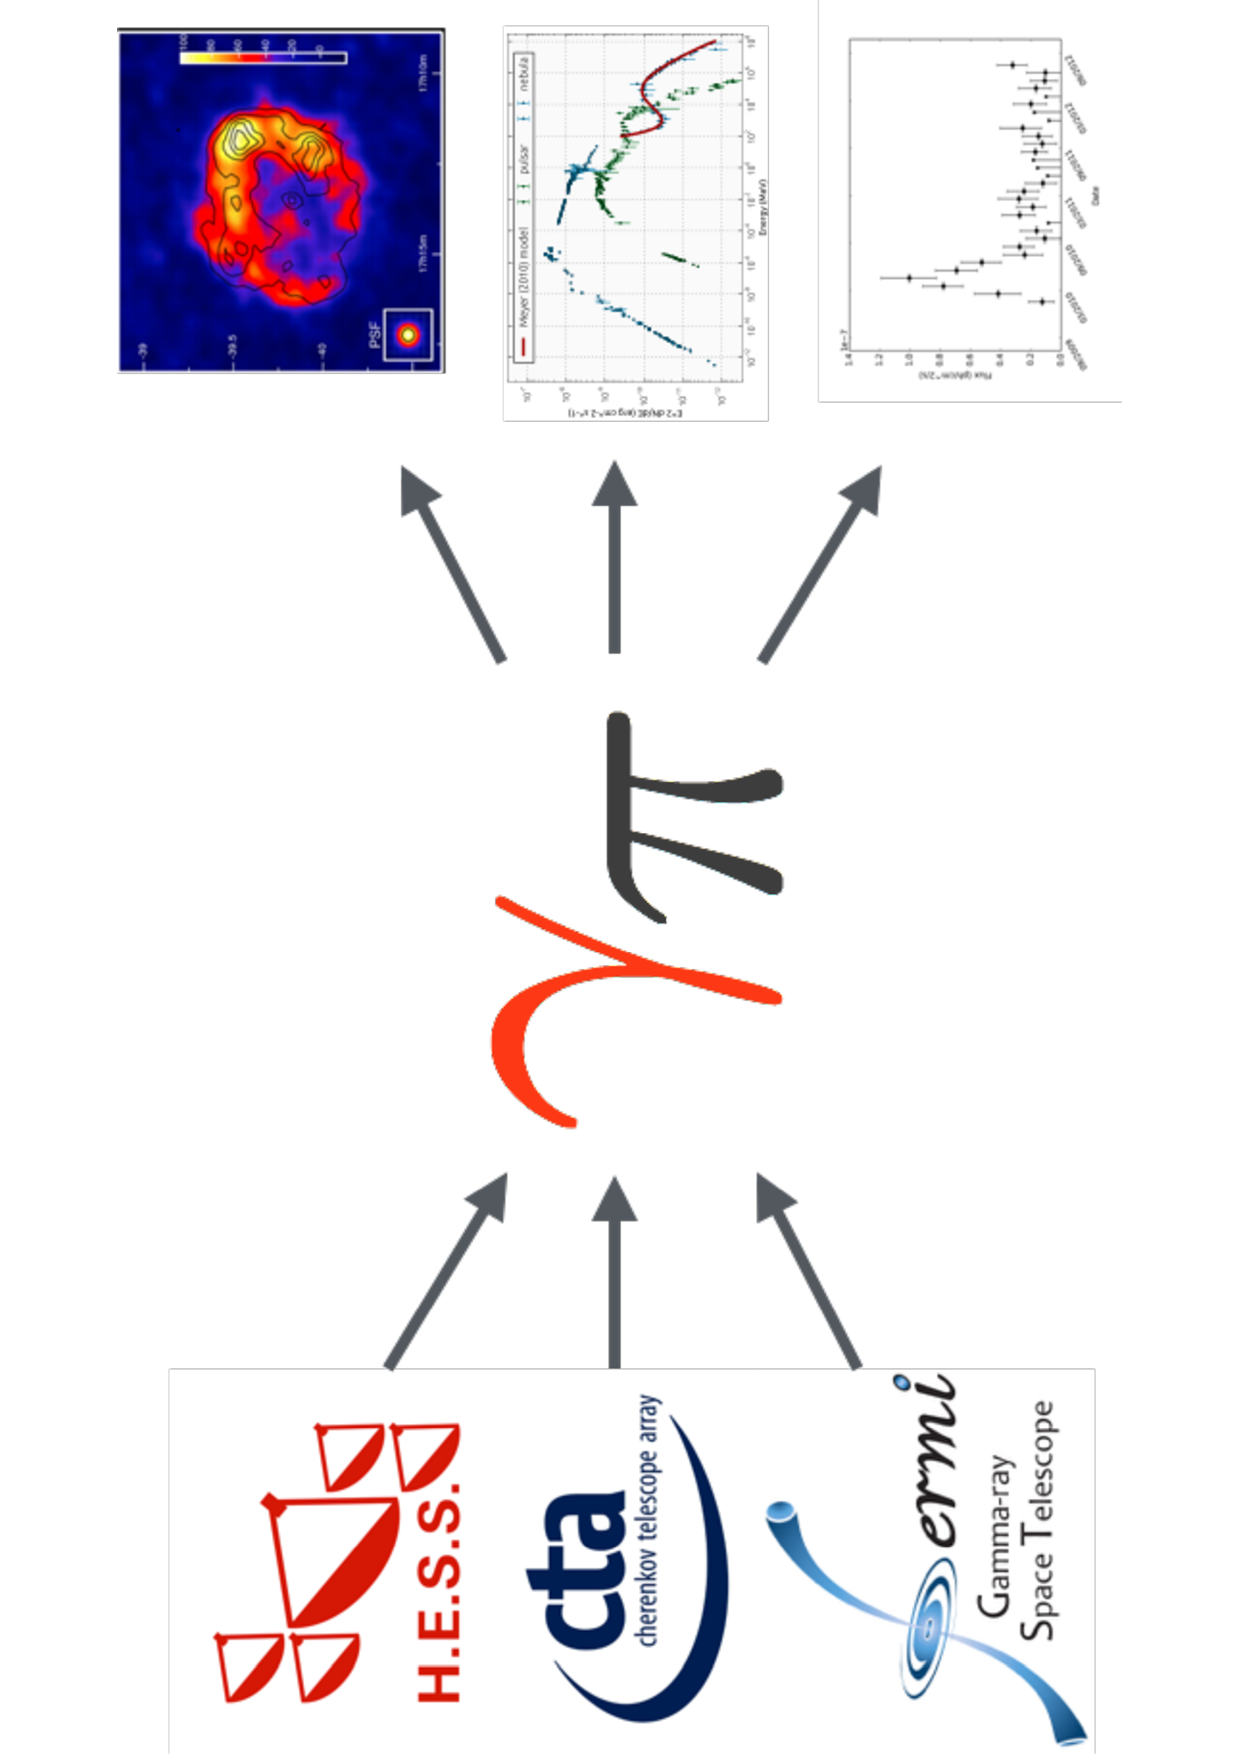
\includegraphics[height=\textwidth, angle=270]{static/gammapy-big-picture}
    \caption{ Gammapy is a Python package
		for high-level gamma-ray data analysis. Using event lists, exposures and point
		spread functions as input you can use it to generate science results such as
		images, spectra, light curves or source catalogs. So far it has been used to
		simulate and analyse H.E.S.S., CTA,  and \textit{Fermi}-LAT data. As demonstrated
		by several studies, it will also be applied to e.g., VERITAS, MAGIC or HAWC data
		in the future. }
	\label{fig:big-picture}

\end{figure*}

Water Cherenkov observatories detect directly particles from the tail of the
shower when it reaches the ground. These instruments have very
large field-of-view, large duty-cycle but higher energy threshold and
usually have lower signal to noise ratios compared to IACTs.

%% Context
Ground based gamma-ray astronomy has been historically structured
by experiments run by independent collaborations relying
on their own proprietary data and analysis software developed as part of the
instrument. While this model has been very successful so far, it does not
permit easy combination of data from several instruments and is therefore
a limitation for interoperability of existing facilities. Especially
because the different detection techniques have complementary
properties.

%TODO: better transition into context
The Cherenkov Telescope Array (CTA) will be the first instrument to be operated
as an open observatory in the domain. Its high level data will be shared publicly after
some proprietary period and the software required to analyze it will be distributed
as well. To allow the re-usability of existing instruments and their interoperability
requires open data formats and open tools that can support the various analysis methods
commonly used in the field.


%% Context : formats
In practice, the data-reduction workflow of all gamma-ray observatories
is remarkably similar.
After data calibration, shower events are reconstructed and
gamma/hadron separation is applied to build lists of gamma-ray like events.
The latter are then used to derive scientific results, such as spectra, sky maps
or light curves, taking into account the specific instrument response functions (IRF).
The information in this high data level is independent on
the data reduction, and eventually of the detection technique. This implies,
for example, that data from IACT and particle samplers can be represented
within the same model. The efforts to prototype a format usable by various instruments
converged in the so-called \textit{Data Format for Gamma-ray Astronomy}
initiative~\citep{gadf_proc, gadf_universe}, abbreviated in
\texttt{gamma-astro-data-format} (GADF). The latter proposes prototypical
specifications to produce files based on the flexible image transport system
(FITS) format~\citep{fits} encapsulating this high-level information. This is
realized by storing a list of gamma-like events with their measured quantites
(energy, direction, arrival time) and a parametrisation of the response of the
system. (see Sec.~\ref{ssec:gammapy-data} and Sec.~\ref{ssec:gammapy-irf} for
more information).

%% Context: develoment of open software
Python has become extremely popular as a scientific programming language
in particular in the field of data sciences. The success is
mostly attributed to the simple and easy to learn syntax, the ability to act as
a "glue" language between different programming languages and last but not least
the rich eco-system of packages and its open and supportive community, from
core numerical analysis packages such as numpy \citep{numpy} and
scipy \citep{2020SciPy-NMeth}, visualization libraries,e.g. matplotlib \citep{matplotlib},
or optimization packages such as iminuit \citep{iminuit}.

The \astropy~\citep{astropy} was created in 2012 to build a community-developed
python package for astronomical reasearch. Among other things, the it offers functionality for
transforming and representing astronomical coordinates, manipulating physical quantities
and their units as well as reading and writing FITS files.

%% Gammapy: concept and goals
%%% Question: starting date? Is is relevant, what is the real start?
The Gammapy project started in 2015 with the objective of building a flexible and
efficient software library for very high energy gamma-ray data analysis \citep{gammapy_2015}.
This is possible thanks to the definition of a common data format such as GADF, and thanks to
an open development with a broad community of contributors.

%Gammapy is built on the scientific Python stack and makes use of Astropy.


%% Gammapy: from first developments to validation and selection
The H.E.S.S. collaboration released a limited test dataset (about 50 hours of
observations taken between 2004 and 2008) based  on the GADF DL3 format \citep{HESS_DR1}.
This data release served as a basis for analysis tools validation \cite[see e.g.]{Mohrmann2019}.

TODO: Figure 1: Data -> Gammapy -> Spectra etc with some details

%% Paper outline
In this article, we describe the general structure of the Gammapy package and
its main concepts. In Section \ref{sec:analysis-workflow-overview}, we present
the data analysis workflow in very high energy gamma-ray astronomy. Then we
show how this workflow is reflected in the structure of the Gammapy package and
describe the various subpackages it contains. Section \ref{sec:applications}
presents a number of applications, while Section \ref{sec:gammapy-project}
discusses the project organization.



\section{Analysis Workflow Overview}

\section{Gammapy package}
\label{sec:package}

The \gammapy package is structured into multiple sub-packages which mostly
follow the stages in the data reduction workflow.

\subsection{Overview}
\begin{figure*}[t]
	\centering
	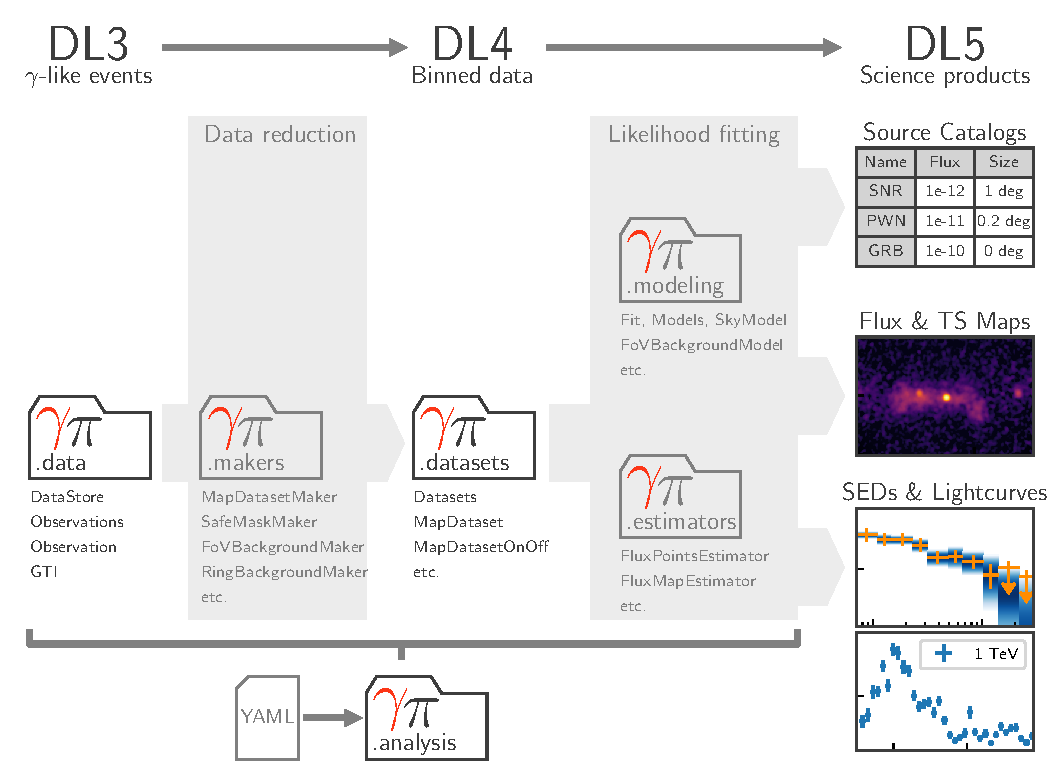
\includegraphics[width=1.\textwidth]{static/data-flow-gammapy}
	\caption{
		Gammapy sub-package structure and data analysis workflow. }
	\label{fig:workflow} \end{figure*}

\subsection{gammapy.data}
The \verb|gammapy.data| sub-package provides access to DL3 level data and
observation handling.

\begin{figure}

	\import{code-examples/generated/}{gp_data}

	\caption{Using gammapy.data to access DL3 level data with a DataStore}
	\label{fig*:minted:gp_data}
\end{figure}

\subsection{gammapy.makers}
\todo{Regis Terrier}
Data reduction

\begin{figure}
	\import{code-examples/generated/}{gp_makers}

	\caption{Using gammapy.data to access DL3 level data}
	\label{ig*:minted:gp_makers}
\end{figure}

\subsection{gammapy.datasets}
\todo{Atreyee Sinha}
DL4 level data

\begin{figure}

	\import{code-examples/generated/}{gp_datasets}
	\caption{Using gammapy.data to access DL3 level data with a DataStore}
	\label{fig*:minted:gp_datasets}
\end{figure}

\subsection{gammapy.modeling}
\todo{Quentin Remy}
Models and fitting

\begin{figure}
	\import{code-examples/generated/}{gp_models}
	\caption{Using gammapy.modeling.models}
	\label{fig*:minted:gp_models}
\end{figure}

\subsection{gammapy.estimators}
\todo{Axel Donath}
Estimators

\subsection{gammapy.visualisation}
Plotters etc.

\subsection{gammapy.analysis}
\todo{Jose Enrique writes this...}
High level analysis API

\subsection{gammapy.astro}
Dark matter models, source population modelling

\subsection{gammapy.data}
\todo{Cosimo Nigro}

\subsection{gammapy.catalog}
Gamma-ray catalog access

\begin{figure}
	\import{code-examples/generated/}{gp_catalogs}
	\caption{Using gammapy.catalogs}
	\label{codeexample:data}
\end{figure}

\subsection{gammapy.maps}
\todo{Laura Olivera-Nieto}
The \verb|gammapy.maps| sub-package provides classes for representing pixelized
data structures with at least two spatial dimensions representing a set of
coordinates or a region on a sphere. In addition it allows to handle and
arbitray  number of non-spatial data axes, such as time or energy.

It provides a uniform API for WCS, HEALPix and region based data structures.

\begin{figure}

	\import{code-examples/generated/}{gp_maps}
	\caption{Using gammapy.data to access DL3 level data with a DataStore}
	\label{codeexample:data}
\end{figure}

\subsection{gammapy.irf}
\todo{Fabio Pintore}
IRF classes

\subsection{gammapy.stats}
\todo{Regis Terrier}
Statistics methods

\subsection{gammapy.utils}
Utility functions...

Outline: * List typical analysis use cases * Can use from Python and Jupyter ->
show Figure with Jupyter notebook here. * Gammapy code structure * How Numpy
and Astropy is used

Figures: * Add a Figure showing dataflow in a typical application DL3 at the
top, spectrum, map, lightcurve, fit results at the bottom. Mention major
classes in between (DataStore, EventList, Map, MapMaker, MapFit, …) * Probably
not: Figure showing sub-packages and how they relate (gammapy.data and
gammapy.irf at the base, then gammapy.maps, etc. * The code example Figure how
to make a counts map, to explain how the package works.

\section{Applications}
\label{sec:applications}

Gammapy can be used for a variety of science cases by different IACT experiments. (Refer to publications)
In this section, we show a non-exhaustive list of some typical analysis that can be performed.
In general from the \gammapy side there is not limitation on which kind of analysis can be
done with wich instrument, however in practice it is limited by the availability of public data.

\subsection{1D Analysis}
\label{ssec:1d-analysis}
\todo{Axel}
One of the most common analysis cases in gamma-ray astronomy is measuring the
spectrum of a source in a given region defined on the sky, in conventional
astronomy also called aperture photometry.
The spectrum is typically measured in two steps: first a parametric
spectral model is fitted to the data and secondly flux points are computed
in a pre-defined set of energy bins.
The result of such an analysis performed on three simulated CTA observations
is shown in Fig.~\ref{fig:cta_galactic_center}.
In this case the spectrum was measured in a circular aperture centered
on the Galactic Center, in \gammaray~astronomy often called "on region".
For such analysis the users first chooses a region of interest
and energy binning, both defined by a `RegionGeom`.
In a second step the events and instrument response are binned into
maps of this geometry, by the `SpectrumDatasetMaker`.
All the data and reduced instrument response are bundled into a
`SpectrumDataset`.
To estimate the expected background in the on region a "reflected regions"
background method was used~\cite{Berge07}, represented in \gammapy
by the `ReflectedRegionsBackgroundMaker` class.
The resulting reflected regions are illustrated for all three observations
on top of the map of counts.
After reduction of the data it was modelled using a forward-folding
method and a power-law spectral shape, using the `PowerLawSpectralModel`
and `Fit` class.
Based on this best fit model the final flux points and
corresponding log-likleihood profiles are computed using
the `FluxPointsEstimator`.

\begin{figure*}[t]
	\centering
	\includegraphics[width=1.\textwidth]{figures/cta_galactic_center.pdf}
	\caption{
        Example spectral analysis of the Galactic Center for three simulated CTA observations.
        The left image shows the maps of counts with the measurement region and background
        regions overlaid in different colors. The right image shows the resulting spectral
        points and their corresponding log-likelihood profiles.
    }
	\label{fig:cta_galactic_center}
\end{figure*}


\subsection{3D Analysis}
\label{ssec:3d-analysis}
\todo{Laura}
The 1D analysis approach is a powerful tool to measure the spectrum of an
isolated source. However, more complicated situations require a more careful
treatment. In a field of view containing several overlapping sources, the 1D
approach can't disentangle the contribution of each source to the total flux in
the selected region. Sources with extended or complex morphology can result in
the measured flux being underestimated, and heavily dependent on the choice of
extraction region. Additionally, the 1D approach neglects the energy-dependence
of the PSF.

For such situations a more complex approach is needed, the so-called 3D
analysis. The three relevant dimensions are the two spatial angular coordinates
and an energy axis. In this framework, a combined spatial and spectral model
(that is, a SkyModel, see Section~\ref{ssec:gammapy-modeling}) is fitted to the
sky-maps that were previously derived from the data and bundled into a
MapDataset (see Sections~\ref{ssec:gammapy-makers} and~\ref{ssec:gammapy-datasets}).

A thorough description of the 3D analysis approach and multiple examples that
use \gammapy can be found in~\cite{Mohrmann2019}. Here we present a short
example to highlight some of its advantages.

Starting from the \irfs corresponding to the same three simulated \cta
observations used in Section~\ref{ssec:1d-analysis}, we can create a MapDataset
via the MapDatasetMaker. However, we will not use the simulated event lists
provided by \cta but instead, use the method MapDataset.fake() to simulate
measured counts from the combination of several SkyModel instances. In this
way, a DL4 dataset can directly be simulated. In particular we simulate:
\begin{enumerate} \item A point source located at (l=0\textdegree, b=0\textdegree) with a power-law
	      spectral shape. \item An extended source with Gaussian morphology located at (l=0.4\textdegree,
	      b=0.15\textdegree) with $\sigma$=0.2\textdegree and a log-parabola spectral
	      shape. \item A large shell-like structure centered around (l=0.06\textdegree,
	      b=0.6\textdegree) with a radius and width of 0.6\textdegree and 0.3\textdegree
	      respectively and a power-law spectral shape. \end{enumerate} The position and sizes of the sources
have been selected so that their contributions overlap. This can be clearly
seen in the significance map shown in the left panel of
Figure~\ref{fig:cube_analysis}. This map was produced with the
ExcessMapEstimator (see Section~\ref{ssec:gammapy-estimators}) with a
correlation radius of 0.1\textdegree.

We can now fit the same model shapes to the simulated data and retrieve the
best-fit parameters. To check the model agreement, we compute the residual
significance map after removing the contribution from each model. This is done
again via the ExcessMapEstimator. As can be seen in the middle panel of
Figure~\ref{fig:cube_analysis}, there are no regions above or below 5$\sigma$,
meaning that the models describe the data sufficiently well.

As the example above shows, the 3D analysis allows to characterize the
morphology of the emission and fit it together with the spectral properties of
the source.  Among the advantages that this provides is the ability to
disentangle the contribution from overlapping sources to the same spatial
region. To highlight this, we define a circular RegionGeom of radius
0.5\textdegree~ centered around the position of the point source, which is drawn
in the left panel of Figure~\ref{fig:cube_analysis}. We can now compare the
measured excess counts integrated in that region to the expected relative
contribution from each of the three source models. The result can be seen in the left
panel of Figure~\ref{fig:cube_analysis}.

\begin{figure*}[t]
	\centering
	\includegraphics[width=1.\textwidth]{figures/cube_analysis.pdf}
	\caption{Example 3D analysis for simulated sources using the \cta \irfs. The
		left image shows a significance map where the three simulated sources can be
		seen. The middle figure shows another significance map, but this time after
		subtracting the best-fit model for each of the sources, which are displayed in
		black. The right figure shows the contribution of each source model to the
		circular region of radius 0.5\textdegree drawn in the left image, together with
		the excess counts inside that region. } \label{fig:cube_analysis} \end{figure*}

Note that all the models fitted also have a spectral component, from which flux
points can be derived in a similar way as described in~\ref{ssec:1d-analysis}.
%\end{figure*}%	\caption{Fermi-LAT TS map in two energy bands} \label{fig:fermi_ts_map}%	\includegraphics[width=1.\textwidth]{figures/fermi_ts_map.pdf}%Ref:~\citep{Stewart2009} \begin{figure*}[t] \centering%\todo{What to do with } Figure~\ref{fig:fermi_ts_map} ?%

\subsection{Temporal analysis}
\label{ssec:temporal-analysis}
A common use case in most astrophysical scenarios is to study the temporal
variability of the source. The most basic way to do this is to construct a
lightcurve, i.e., the flux of the source in each given time bin. In \gammapy, this
is done by using the \code{LightCurveEstimator} which fits the normalisation of the
source in each energy band per observation, keeping other parameters constant.
For custom time binning, an observation needs to be split into finer time bins using
the \code{Observation.select\_time} method. Figure~\ref{fig:hess_lightcurve_pks}
shows the lightcurve of the blazar PKS~2155-304 in different energy bands as
observed by the H.E.S.S. telescope during an exceptional flare on the night of
July 29 - 30, 2006~\cite{2009A&A...502..749A}. The data is available publicly
as a part of the HESS-DL3-DR1~\cite{HESS-DL3-DR1}, and shipped with
\verb"GAMMAPY_DATA". Each observation is first split into 10 min smaller
observations, and spectra extracted for each of these within a 0.11 deg radius
around the source. A \code{PowerLawSpectralModel} is fit to all the datasets, leading
to a reconstructed index of $3.54 \pm 0.02$. With this assumed spectral model
the \code{LightCurveEstimator} runs directly for two energy bands, 0.5 - 1.5
TeV, and 1.5 - 20 TeV, respectively.
%
\begin{figure*}[t]
	\centering
	\includegraphics[width=0.6666\textwidth]{figures/hess_lightcurve_pks.pdf}
	\caption{10 min binned lightcurve for PKS~2155-304 in two energy bands, (500
		GeV - 1.5 TeV, and 1.5 TeV to 20 TeV) as observed by the H.E.S.S. telescopes in
		2006.} \label{fig:hess_lightcurve_pks}
\end{figure*}
%
The obtained flux points can be analytically modelled using the available, or
user-implemented temporal models. Alternatively, instead of  extracting a
lightcurve, it is also possible to directly fit temporal models to the reduced
datasets. By associating an appropriate \code{SkyModel}, consisting of both temporal
and spectral components, or using custom temporal models with spectroscopic
variability, to each dataset, a joint fitting across the datasets will directly
return the best fit temporal and spectral parameters.

\subsection{Multi instrument analysis}
\label{ssec:multi-instrument-analysis}
\todo{Cosimo Nigro}


\begin{figure*}[t]
	\sidecaption
	\includegraphics[width=0.666\textwidth]{figures/multi_instrument_analysis.pdf}
	\caption{A multi-instrument analysis of the Crab Nebula}
	\label{fig:multi_instrument_analysis}
\end{figure*}

\subsection{Broadband SED Modeling}
\label{ssec:broadband-sed-modeling}
Figure \ref{fig:multi_instrument_analysis}. Add explanation text.

\subsection{Surveys, catalogs, and population studies}
\label{ssec:surveys-catalogs-and-population-studies}

Sky surveys have a large potential for new source detections, and new phenomena
discovery. They also offer less selection bias to perform source population
studies over a large set of coherently detected and modelled objects. Early
versions of \textit{gammapy} were developed in parallel of the preparation of
the \hess Galactic plane survey catalog~\citep[HGPS][]{2018A&A...612A...1H} and
the associated PWN and SNR populations studies~\citep{2018A&A...612A...2H,
	2018A&A...612A...3H}.

The increase in sensitivity  and resolution provided by new generation of
instruments scale up the number of sources detectable and the complexity of the
models needed to represent them accurately. As an example If we compare the
results of the HGPS to the expectations from the \cta Galactic Plane survey
simulations we jump from 78 sources detected by \hess to about 500 detectable by
CTA~\citep{2021arXiv210903729R}.

Studies performed on simulations not only offer a first glimpse on what could
be the sky seen by CTA (according to our current knowledge on source
populations), but also give us the opportunity to test the software on complex
use cases\footnote{Note that the CTA-GPS simulations were performed with the
	\textit{ctools} package~\citep{2016A&A...593A...1K} and analysed with both
	\textit{ctools} and \textit{gammapy} packages in order to cross-validate
	them.}. So we can  improve performances, optimize our analyses strategies, and
identify the needs in term of parallelisation to process the large datasets
provided by the surveys.

In short the production of catalogs from \gammaray surveys can be divided in
four main steps : data-reduction; object detection; model fitting and model
selection; associations and classification. The IACTs data-reduction step is
done in the same way than described in the previous sections but scale-up to
few thousand of observations. The object detection step consists a minima in
finding local maxima in the significance, or TS maps,  given by the
ExcessMapEstimator, or TSMapEstimator, respectively.  Further refinements can
include for example  filtering and detection on these maps with techniques from
scikit-image package~\citep{scikit-image}, and outlier detection from
scikit-learn package~\citep{scikit-learn}. Tests on simulations shown that it
reduces the spurious detections at this stage and then speed up the next step
as less objects will have to be fitted simultaneously. During the modelling
step each object is alternatively fitted with different models in order to
determine their optimal parameters, and the best-candidate model. The
subpackage gammapy.modeling.models offers a large variety of choice, and the
possibility to add custom models.  Several spatial models (point-source, disk,
gaussian...), and spectral models (power-law, log-parabola...) may be tested
for each object, so the complexity of the problem increases rapidly in regions
crowded with multiple extended sources. Finally an object is discarded if its
best-fit model is not significantly preferred over the null hypothesis (no
source) comparing the difference in log-Likelihood between these two
hypotheses. For the association and classification step, that is tightly
connected to the population studies, we can a minima compare the fitted models
to the set of gammapy-ray catalogs available in gammapy.catalog. However
further multi-wavelength cross-matches are usually required to characterize the
sources.



\section{Gammapy project}
\label{sec:gammapy-project}

In this section, we provide an overview of the organization of the Gammapy project. We briefly describe the main roles and responsibilities within the team, as well as the technical infrastructure designed to facilitate the development and maintenance of Gammapy as a high quality software. We use common tools and services for software development of Python open-source projects, code review, testing, package distribution and user support, with a customized solution for a versioned thoroughly tested documentation in the form of user-friendly playable recipes. This section concludes with an outlook on the roadmap for future directions.

\subsection{Organizational structure}
\label{ssec:organizational-structure}

Gammapy is a well-organised international open-source project with a broad developer base and the presence of commitments from strong groups and institutes in the very high-energies astrophysics domain \footnote{\url{https://gammapy.org/team.html}}. The main development roadmaps are discussed and validated by a Coordination Committee, composed of representatives of the main contributing laboratories. This committee is chaired by a Project Manager and his deputy while two Lead Developers manage the development strategy and organise technical activities. Because of this institutionally driven characteristic, the permanent staff and commitment of supporting institutes ensure the continuity of the executive teams. A core team of developers from the contributing laboratories is in charge of the regular development, which benefits from punctual contributions of the community at large.

\subsection{Technical infrastructure}
\label{ssec:technical-infrastructure}

Gammapy follows an open-source and open-contribution development model based on the cloud repository service GitHub. A GitHub organization \textit{gammapy} \footnote{\url{https://github.com/gammapy}} hosts different repositories related with the project. The software codebase may be found in the \textit{gammapy} repository (see Table~\ref{table:codestats:data} and Figure~\ref{fig:codestats:lang} for code lines statistics). We make extensive use of the pull request system to discuss and review code contributions.

\begin{table}
	\import{tables/generated/}{codestats}
	\caption{Coding languages statistics in Gammapy project}
	\label{table:codestats:data}
\end{table}

\begin{figure}[t]
	\centering
	\includegraphics[width=0.5\textwidth]{figures/codestats.pdf}
	\caption{
		Percentage of lines of code in Gammapy project} \label{fig:codestats:lang}
\end{figure}

Several automatized tasks are set as GitHub actions \footnote{\url{https://github.com/features/actions}}, blocking the processes and alerting developers when fails occur. This is the case of the content integration workflow, which monitors the execution of the test coverage suite \footnote{\url{https://pytest.org}} using datasets from the \textit{gammapy-data} repository. Tests scan not only the codebase but also the code snippets present in docstrings of the scripts and in the RST documentation files, as well as in the tutorials provided in the form of Jupyter notebooks. 

Other automatized tasks, executing in the \textit{gammapy-benchmarks} repository, are responsible for numerical validation tests and benchmarks monitoring. Also tasks related with the release process are partially automatized, and every contribution to the codebase repository triggers the documentation building and publishing workflow within the \textit{gammapy-docs} repository (see Sec. ~\ref{ssec:software-distribution} and Sec. ~\ref{ssec:documentation}).

This small ecosystem of interconnected up-to-date repositories, automatized tasks and alerts, is just a part of a bigger set of GitHub repositories, where most of them are related with the project but not necessary for the development of the software (i.e. project webpage, complementary high-energy astrophysics object catalogs, coding sprints and weekly developer calls minutes, contributions to conferences, other digital assets, etc.) Finally, third-party services for code quality metrics are also set and may be found as status shields in the codebase repository.

\subsection{Software distribution}
\label{ssec:software-distribution}

\begin{itemize}
	\item pip, conda, versions
	\item gammapy download
	\item automated release process with Zenodo publishing linking
	\item escape 2020 software platform
	\item ascl
\end{itemize}

\subsection{Documentation}
\label{ssec:documentation}

\begin{itemize}
	\item rst, sphinx, api
	\item versioned notebooks building and testing
	\item versioned binder
\end{itemize}

\subsection{Community and user-support}
\label{ssec:community-and-user-support}

\begin{itemize}
	\item web and on-line documentation 	
	\item slack
	\item github discussions
	\item weekly developers calls
	\item coding sprints 
	\item gammapy recipes repo
	\item mailing lists 
		\begin{verbatim}
		gammapy-coordination-l@in2p3.fr 
		gammapy@googlegroups.com 
		gammapy-cta-l@in2p3.fr
		\end{verbatim}
	\item twitter
\end{itemize}

\subsection{Roadmap}
\label{ssec:roadmap}
\todo{Axel, Regis}

\begin{itemize}
	\item pigs
	\item roadmap
\end{itemize}

\section{Summary and Outlook}
\label{sec:summary-and-outlook}

\todo{Axel and Regis write this...}

Summary what we have in v0.9 and presented in this paper.

Roadmap to v1.0, about half a page.

Short conclusion: Gammapy has potential to be the Python package for gamma-ray
astronomy.

Prospects for HAWC / SWGO? Or speak in general about water Cherenkov
observatories...
\begin{acknowledgements}

	Mention Christoph here?

	We would like to thank the \texttt{Numpy}, \texttt{Scipy}, \texttt{IPython} and
	\texttt{Matplotlib} communities for providing their packages which are
	invaluable to the development of Astropy. We thank the \github team for
	providing us with an excellent free development platform. We also are grateful
	to Read the Docs (\ReadthedocsUrl), and Travis (\TravisUrl) for providing free
	documentation hosting and testing respectively. Finally, we would like to thank
	all the \gammapy users that have provided feedback and submitted bug reports.

	TODO: copy over stuff from
	\url{http://docs.gammapy.org/en/latest/about.html#thanks}.

	TODO: add the ANR for Luca (and Atreyee in LUPM?)

	J.E. Ruiz acknowledges financial support from the State Agency for Research of
	the Spanish MCIU through the "Center of Excellence Severo Ochoa" award to the
	Instituto de Astrof\'isica de Andaluc\'ia (SEV-2017-0709)

\end{acknowledgements}


% Back matter
\bibliographystyle{aa}
\bibliography{bib.bib}

\end{document}
